\chapter{Implementácia}
\label{kap:implementacia}

V kapitole opisujeme priebeh vzniku aplikácie, implementačné detaily, postupy a rozhodnutia. Základné členenie obsahu je podľa modulov, za ktoré považujeme celky aplikácie ako editor kódu v grafickom jazyku, modul pre sériovú komunikáciu či modul pre simuláciu. V rámci jednotlivých častí je opísaný ich vývoj pokiaľ možno chronologicky. Súčasťou sú tiež implementačne zmeny v riadiacich programoch robotov.

\section{Desktopová aplikácia}
Vývoj sme začali návrhom kostry a vizuálnej podoby aplikácie, v ktorej neskôr vznikli jednotlivé moduly. V prvej fáze sme implementovali časti podporujúce komunikáciu s aktuálnou verziou riadiaceho programu robota Otto a jeho programovanie. Nasledovala etapa rozširovania funkcionalít (hlavne grafického jazyka) tak, aby sme sa čo v najväčšej miere vyrovnali existujúcim programom. Súčasne sa zameriavame na modul simulácie.

\subsection{Grafické rozhranie}
- radz od konštruktérov Blockly (rozloženie)
todo

\subsection{Editor kódu}
aka blokové paradigmy, odporúčania tvorcov, uvedomiŤ si kto je publikum, šetriť s počtom blokov, zobraziť len tie čo sa aktuálne dajú použiť

\subsubsection{Obrazový programovací jazyk}
- granularita puzzle
- pre rozne vekove kategorie (na zaklade poziadaviek)
- premenne - problem s typmi

\subsection{Komunikácia s robotom}
todo

\subsubsection{Upload programu}
todo

\subsubsection{Komunikácia cez konzolu}
todo, to co poskytuje putty alebo Arduino IDE, alebo OttoBlockly

\subsection{Kompilácia}
todo

\subsection{Vizualizácia}
todo, tinkerpad, 3d tlac - existujuce modely
- 1.pokus: zobrazenie fixne, rotacia jednotlivych casti
- problemy s fyzikou, komplexita mesh collision shape -> riesenie je boxCollisionShape
- jonts = servo?
- obrazky - motor 130 deg.

\begin{figure}
\centerline{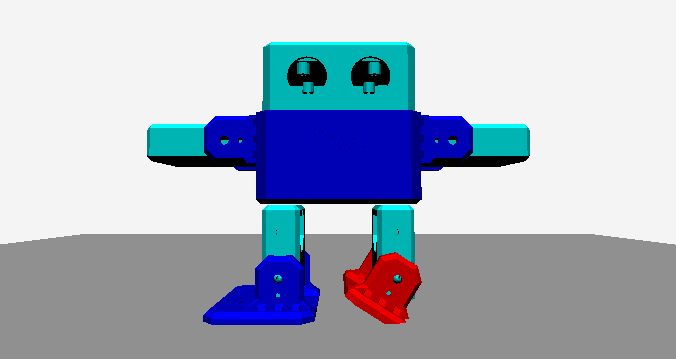
\includegraphics[width=0.4\textwidth]{images/otto-without-collision}}
\caption[Robot Otto - simulácia bez detekcie kolízií]{Robot Otto - simulácia bez detekcie kolízií}
\label{obr:otto-without-collision}
\end{figure}

\begin{figure}
\centerline{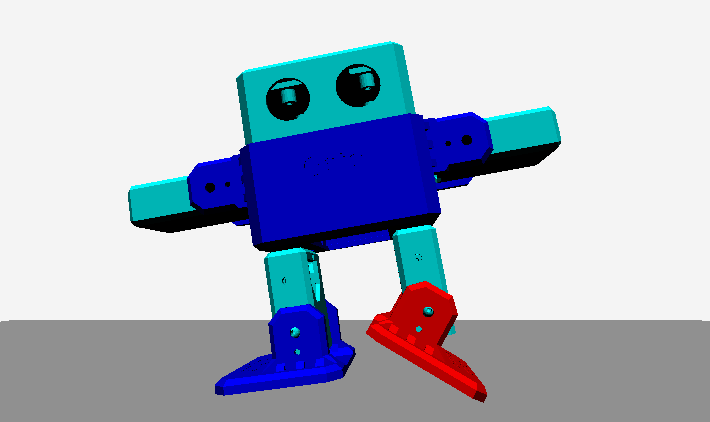
\includegraphics[width=0.4\textwidth]{images/otto-with-collision}}
\caption[Robot Otto - simulácia s detekciou kolízií]{Robot Otto - simulácia s detekciou kolízií}
\label{obr:otto-with-collision}
\end{figure}

\section{Riadiaci program robota}
todo

\subsection{Robot Otto}
todo

\subsection{Robot Mokrarosa}
todo
